%%%%%%%% ICML 2018 EXAMPLE LATEX SUBMISSION FILE %%%%%%%%%%%%%%%%%

\documentclass{article}

% Recommended, but optional, packages for figures and better typesetting:
\usepackage{microtype}
\usepackage{graphicx}
\usepackage{subfigure}
\usepackage{booktabs} % for professional tables

% Added by wenlong lyu
\usepackage{amsmath}
\usepackage[plain]{fancyref}
\usepackage{bm}
\usepackage{todonotes}
\usepackage{placeins}
\usepackage{multirow}

% hyperref makes hyperlinks in the resulting PDF.
% If your build breaks (sometimes temporarily if a hyperlink spans a page)
% please comment out the following usepackage line and replace
% \usepackage{icml2018} with \usepackage[nohyperref]{icml2018} above.
\usepackage{hyperref}

% Attempt to make hyperref and algorithmic work together better:
\newcommand{\theHalgorithm}{\arabic{algorithm}}

% % Use the following line for the initial blind version submitted for review:
% \usepackage{icml2018}

% If accepted, instead use the following line for the camera-ready submission:
\usepackage[accepted]{icml2018}

% The \icmltitle you define below is probably too long as a header.
% Therefore, a short form for the running title is supplied here:
\icmltitlerunning{Supplemental Materials}

\begin{document}

\twocolumn[
\icmltitle{Supplemental Materials}

% It is OKAY to include author information, even for blind
% submissions: the style file will automatically remove it for you
% unless you've provided the [accepted] option to the icml2018
% package.

% List of affiliations: The first argument should be a (short)
% identifier you will use later to specify author affiliations
% Academic affiliations should list Department, University, City, Region, Country
% Industry affiliations should list Company, City, Region, Country

% You can specify symbols, otherwise they are numbered in order.
% Ideally, you should not use this facility. Affiliations will be numbered
% in order of appearance and this is the preferred way.
% \icmlsetsymbol{equal}{*}

% \begin{icmlauthorlist}
%     \icmlauthor{Wenlong Lyu}{fudan}
%     \icmlauthor{Fan Yang}{fudan}
%     \icmlauthor{Changhao Yan}{fudan}
%     \icmlauthor{Dian Zhou}{fudan,utd}
%     \icmlauthor{Xuan Zeng}{fudan}
% % \icmlauthor{Aeiau Zzzz}{equal,to}
% % \icmlauthor{Bauiu C.~Yyyy}{equal,to,goo}
% % \icmlauthor{Cieua Vvvvv}{goo}
% % \icmlauthor{Iaesut Saoeu}{ed}
% % \icmlauthor{Fiuea Rrrr}{to}
% % \icmlauthor{Tateu H.~Yasehe}{ed,to,goo}
% % \icmlauthor{Aaoeu Iasoh}{goo}
% % \icmlauthor{Buiui Eueu}{ed}
% % \icmlauthor{Aeuia Zzzz}{ed}
% % \icmlauthor{Bieea C.~Yyyy}{to,goo}
% % \icmlauthor{Teoau Xxxx}{ed}
% % \icmlauthor{Eee Pppp}{ed}
% \end{icmlauthorlist}

% % \icmlaffiliation{utd}{utdallas}
% \icmlaffiliation{fudan}{State Key Lab of ASIC and System, Microelectronics Department, Fudan University, Shanghai, China}
% \icmlaffiliation{utd}{Department of Electrical Engineering, University of Texas at Dallas, Richardson, TX, U.S.A}
% % \icmlaffiliation{to}{Department of Computation, University of Torontoland, Torontoland, Canada}
% % \icmlaffiliation{goo}{Googol ShallowMind, New London, Michigan, USA}
% % \icmlaffiliation{ed}{School of Computation, University of Edenborrow, Edenborrow, United Kingdom}

\icmlcorrespondingauthor{Xuan Zeng}{xzeng@fudan.edu.cn}
% \icmlcorrespondingauthor{Eee Pppp}{ep@eden.co.uk}

% You may provide any keywords that you
% find helpful for describing your paper; these are used to populate
% the "keywords" metadata in the PDF but will not be shown in the document
\icmlkeywords{Bayesian Optimization, Automated analog circuit design}

\vskip 0.3in
]

% this must go after the closing bracket ] following \twocolumn[ ...

% This command actually creates the footnote in the first column
% listing the affiliations and the copyright notice.
% The command takes one argument, which is text to display at the start of the footnote.
% The \icmlEqualContribution command is standard text for equal contribution.
% Remove it (just {}) if you do not need this facility.

% \printAffiliationsAndNotice{}  % leave blank if no need to mention equal contribution
% \printAffiliationsAndNotice{\icmlEqualContribution} % otherwise use the standard text.
\section{Additional Experiments with varied batch sizes}

\subsection{The Analytical Benchmark Functions}

We performed additional experiments with varied batch sizes $B = 2$, $B = 3$ and $B = 5$, the results is shown in \Fref{tab:result_analytical_b2}, \Fref{tab:result_analytical_b3} and \Fref{tab:result_analytical_b5}.

\begin{table*}[!htb]
    \centering
    \caption{Optimization results of the benchmark functions with batch size $B=2$}
    \label{tab:result_analytical_b2}
    \begin{tabular}{llllll}
        \toprule
        Algorithm     & MACE                          & BLCB                       & EI-LP                        & QKG                    & QEI                              \\ \midrule
        Ackley        & 1.15            $\pm$  0.646     &  1.7      $\pm$  0.85      &  \textbf{0.507    $\pm$  0.408}   &  4.31   $\pm$  1.81    &  3.07   $\pm$  0.786     \\
        Alpine1       & \textbf{1.38    $\pm$  0.768}    &  3.23     $\pm$  1.03      &  1.55     $\pm$  0.689       &  3.17   $\pm$  0.749   &  2.4    $\pm$  0.904     \\
        Branin        & \textbf{0.398   $\pm$  1.03e-05} &  0.398    $\pm$  0.000265  &  0.424    $\pm$  0.0395      &  0.607  $\pm$  0.159   &  0.399  $\pm$  0.00156   \\
        Eggholder     & -844            $\pm$  65.4      &  -828     $\pm$  66.2      &  \textbf{-877     $\pm$  51.6}    &  -845   $\pm$  78.3    &  -855   $\pm$  78.4      \\
        Hartmann6     & \textbf{3.27    $\pm$  0.0584}   &  -3.25    $\pm$  0.0587    &  -3.16    $\pm$  0.301       &  -3.07  $\pm$  0.0823  &  -3.14  $\pm$  0.128     \\
        Rosenbrock    & \textbf{0.00105 $\pm$  0.0011}   &  0.00556  $\pm$  0.00928   &  8.37     $\pm$  5.63        &  9.41   $\pm$  10.7    &  10.3   $\pm$  8.52      \\
        Ackley10D     & \textbf{2.75    $\pm$  0.497}    &  3.13     $\pm$  0.723     &  18.5     $\pm$  1.02        &  18.4   $\pm$  0.943   &  18.8   $\pm$  0.608     \\
        Rosenbrock10D & \textbf{223     $\pm$  104}      &  552      $\pm$  223       &  1.1e+03  $\pm$  496         &  957    $\pm$  439     &  757    $\pm$  405       \\
        \bottomrule
    \end{tabular}
\end{table*}

\begin{table*}[!htb]
    \centering
    \caption{Optimization results of the benchmark functions with batch size $B=3$}
    \label{tab:result_analytical_b3}
    \begin{tabular}{llllll}
        \toprule
        Algorithm     & MACE                          & BLCB                       & EI-LP                        & QKG                    & QEI                      \\
        \midrule
        Ackley        & 1.37           $\pm$  1.39      &  1.71         $\pm$  1.02      &  \textbf{0.216  $\pm$  0.148}  &  5.49   $\pm$  1.94   &  2.34   $\pm$  0.788     \\
        Alpine1       & \textbf{1.03   $\pm$  0.746}    &  2.63         $\pm$  1.2       &  1.1    $\pm$  0.376      &  3.18   $\pm$  0.225  &  2.25   $\pm$  0.42      \\
        Branin        & \textbf{0.398  $\pm$  3.18e-05} &  0.398        $\pm$  1.3e-4    &  0.432  $\pm$  0.0183     &  0.645  $\pm$  0.188  &  0.398  $\pm$  0.000135  \\
        Eggholder     & -894           $\pm$  62.9      &  -877         $\pm$  32.2      &  \textbf{-894   $\pm$  43.3}   &  -842   $\pm$  79.2   &  -878   $\pm$  63.1      \\
        Hartmann6     & \textbf{3.31   $\pm$  0.0359}   &  -3.27        $\pm$  0.0584    &  -3.27  $\pm$  0.0531     &  -2.99  $\pm$  0.188  &  -3.13  $\pm$  0.108     \\
        Rosenbrock    & \textbf{9.5e-4 $\pm$  7.8e-4}   &  0.00148      $\pm$  0.00212   &  3.78   $\pm$  3.4        &  4.28   $\pm$  5.5    &  5.44   $\pm$  4.21      \\
        Ackley10D     & 3.05           $\pm$  0.682     &  \textbf{3.05 $\pm$  0.431}    &  17.6   $\pm$  3.53       &  18.5   $\pm$  0.731  &  18.6   $\pm$  0.438     \\
        Rosenbrock10D & \textbf{208    $\pm$  92.5}     &  389          $\pm$  187       &  653    $\pm$  473        &  695    $\pm$  307    &  953    $\pm$  410       \\
        \bottomrule
    \end{tabular}
\end{table*}

\begin{table*}[!htb]
    \centering
    \caption{Optimization results of the benchmark functions with batch size $B=5$}
    \label{tab:result_analytical_b5}
    \begin{tabular}{llllll}
        \toprule
        Algorithm     & MACE                          & BLCB                       & EI-LP                        & QKG                    & QEI                      \\
        \midrule
        Ackley        & 1.7            $\pm$  1.02     &  1.38          $\pm$  0.836    &  \textbf{0.105 $\pm$  0.0978} &  5.27   $\pm$  1.38   &  2.16         $\pm$  1.11  \\
        Alpine1       & \textbf{0.654  $\pm$  0.317}   &  1.68          $\pm$  1.26     &  0.766         $\pm$  0.441   &  3.21   $\pm$  0.497  &  2.05         $\pm$  0.341 \\
        Branin        & \textbf{0.398  $\pm$  1.81e-5} &  0.398         $\pm$  3.42e-05 &  0.412         $\pm$  0.0154  &  0.561  $\pm$  0.163  &  0.398        $\pm$  5.21e-05 \\
        Eggholder     & -886           $\pm$  74.3     &  -899          $\pm$  33.5     &  -896          $\pm$  94.3    &  -889   $\pm$  29.4   &  \textbf{-911 $\pm$  25.8}  \\
        Hartmann6     & -3.27          $\pm$  0.0584   &  \textbf{-3.29 $\pm$  0.0546}  &  -3.27         $\pm$  0.0546  &  -2.85  $\pm$  0.221  &  -3.12        $\pm$  0.105 \\
        Rosenbrock    & \textbf{5.5e-4 $\pm$  8.1e-4}  &  9.4e-4        $\pm$  6.8e-4   &  2.72          $\pm$  1.97    &  3.42   $\pm$  4.8    &  6.69         $\pm$  5.34  \\
        Ackley10D     & \textbf{2.63   $\pm$  0.486}   &  3.05          $\pm$  0.319    &  15.7          $\pm$  5.69    &  18.1   $\pm$  0.476  &  18.1         $\pm$  0.653 \\
        Rosenbrock10D & \textbf{81.9   $\pm$  22.9}    &  348           $\pm$  83.7     &  645           $\pm$  470     &  893    $\pm$  393    &  705          $\pm$  314   \\
        \bottomrule
    \end{tabular}
\end{table*}

% \begin{abstract} 
    Recently, Bayesian optimization has been proposed for automated analog
    circuit design and has shown very good performance. However, the sequential
    property of Bayesian optimization limits its further application. In this
    paper, a batched bayesian optimization method is proposed, the
    parallelization is realized via multi-objective ensemble of acquisition
    functions. In each iteration, multiple acquisition functions are selected,
    multi-objective optimization is then performed to search for the Pareto
    front of the acquisition functions, candidate points are then sampled from
    the Pareto fronts. The proposed method is compared with several
    state-of-the-art algorithms using analytical benchmark functions and
    real-world analog circuits, the experimental results show that the proposed
    method is competitive.
\end{abstract}

% \section{Introduction}

% % TODO: more introduction to the importance of anlog IC sizing, as the reviewers may not have much knowledge of circuit design
Automated analog circuit design has been a challenging problem for the
community of electronic design automation (EDA). Unlike digital circuits, where
the design flow is highly automated, analog circuit design still
heavily relies on designer's experience. The design parameters of analog circuits like
transistor widths and lengths need to be manually calculated based on the
specifications and the designers' understanding of the circuit. However, due to
the ever-scaling IC manufacture technology and the increasing demands for
high-performance, low-power circuits, it is getting much more difficult to meet
the performance and time-to-market requirement with manual circuit design.
Automated analog circuit design has thus attracted more research interests in
the past decade~\cite{rutenbar2007hierarchical}.

% TODO: Traditional methods using offline model and simulated based methods are
% not good
The analog circuit design automation problems can be formulated as optimization
problems, the aim is to find the optimal vector of design parameters that give
best figure of merit (FOM). Prior works about analog circuit optimization
include offline model-based approaches
~\cite{colleran2003optimization,daems2003simulation,wang2014enabling} and
simulation based approaches. The offline model-based methods try to build
accurate global model and then apply global optimization algorithms to the
cheap-to-evaluate models, the model either comes from designers' manual
derivation or from regression models like SVM and ANN. The problem of this
approach is that the accurate models are usually hard to get, for example,
in~\cite{wang2014enabling}, 100,000 randomly simulated points are used to train
a sparse polynomial model for a circuit with ten design parameters.
Simulation-based methods, instead, treat the circuits as black-box functions
that get the objective value from circuit simulations, global optimization
algorithms are directly applied to the black-box functions. For
simulation-based circuit optimization methods, meta-heuristic algorithms like
particle swarm intelligence (PSO)~\cite{phelps2000anaconda} and differential
evolution algorithm (DE)~\cite{liu2009analog} are widely used, although these
algorithm are able to explore the whole design space, they have relatively low
convergence rate and consume many circuit simulations. When the circuit
simulation takes a long time, both model-based and simulation-based approaches
can be prohibitive.

% TODO: Bayesian optimization is a sequential algorithm, there is a need to
% parallelize it
%
% TODO: cite the two 3D-IC papers of TVLSI
To reduce the circuit simulations needed by the optimization, the Gaussian
process (GP)~\cite{GPML} model has been introduced as online surrogate model to
assist the optimization. In~\cite{liu2014gaspad}, GP is combined with
differential evolution algorithm, in~\cite{lyu2017efficient}. Recently, the
Bayesian optimization (BO)~\cite{shahriari2016taking} algorithm has been applied for analog circuit
optimization, the Bayesian optimization algorithm is firstly introduced for the
automated design of general analog circuits, and has shown very good
performance compared to other simulation-based approaches,
in~\cite{wang2017efficient}, the Bayesian optimization algorithm is combined
with adaptive Monte-Carlo sampling to optimize the yield of analog circuits and
static random-access memory (SRAM).

The Bayesian optimization algorithm is a well-studied algorithm, and has
demonstrated to be a promising algorithm for automated analog circuit design,
however, the standard Bayesian optimization algorithm is sequential, it chooses
the next evaluation point by optimizing the specified acquisition fucntion,
which makes the parallelization of Bayesian optimization non-trivial. The
sequential property of BO limits its further application, as multi-core
processors are usually availble for modern computers. 

% TODO: Review current methods
% TODO: See how other papers review existing batched BO methods
Batched Bayesian optimization has been a \textcolor{red}{hot} topic in the BO
literature. Related works include the \emph{simulation matching}
method~\cite{azimi2010batch}, the \emph{BUCB} (BLCB for minimization)
method~\cite{desautels2014parallelizing}, the \emph{GP-UCB-PE}
method~\cite{contal2013parallel}, the \emph{local penalization}
method~\cite{gonzalez2016batch}, the \emph{parallel predictive entropy
search}~\cite{shah2015parallel} and the \emph{qKG}
method~\cite{wu2016parallel}.

% BUCB, UCB-PE: regret bound
% PPES: entropy search
% qKG, qEI: optimal decision if multiple points are selected
% LP: very good heuristic

% TODO: Beiefly introduce my algorithm
All the above mentioned algorithms choose to use one acquisition function, and
except for the smulation mathcing method and local penalization method which
can select arbitrary acquisition function, other parallelization methods rely on
specific acquisition function, the UCB acquisition fucntion must be used for
BUCB and GP-UCB-PE, and the knowledge gradient method must be used for qKG
algorithm. As has been stated in~\cite{hoffman2011portfolio}, no one
acquisition fucntion can always outperform other acquisition functions, so
relying on one acquisition fucntion may resulting in poor performance. Also, a
portfolio strategy that ensembles multiple acquisition functions would be
helpful.

In this paper, we propose to parallize the Bayesian optimization algorithm via
a multi-objective ensemble of acquisition functions. Firstly, in each
iteration, after the GP model is updated, multiple acquisition functions are
selected, we then perform multi-objective optimization to find the \emph{Pareto
front} (PF) of the acquisition functions. The PF represents the best trade-off
between these acquisition functions, when used in sequential mode, the propose
multi-objective acquisition ensemble (MACE) strategy can be seen as a portfolio
strategy, when batched evaluation is possible, we can sample multiple points on
the PF as there are usually much more points on the PF than the batch size.

We tested the MACE algorithm using several analytical benchmark functions and
two real-world analog circuits, including an operational amplifier with
\textcolor{red}{14} design parameters and a class-E power amplifier with
\textcolor{red}{ten} design parameters. The BLCB method, local penalization
method with expected improvement acquisition fucntion (EI-LP), the qEI methods
and qEI methods are compared with MACE. The proposed MACE method achieved
competitive performance when compared with the listed state-of-the-art
algorithms.

% \section{Background}

\textcolor{red}{TODO: See how other people describe GP and BO}

\subsection{Formulation}

We formulate the sizing problem as an optimization problem

\textcolor{red}{TODO: The circuit performance comes from \bf{circuit} simulation}
\textcolor{red}{TODO: format, citation of HSPICE/spectre}

We handle the scenarios that topology of the analog circuit is fixed, this is
practical, as for each task, thare are usually a lot of classical topologies
that can be used. Once the topology is fixed, the designer has to choose the
optimal design parameters according to the specifications and the circuit
device model. What we want to do is to automatically search for the optimal
design parameters, this task can be formulated as a bound-constrained black-box optimization problem:

\begin{equation}
    \label{eq:MOFormulation}
    \text{minimize}~\mathrm{FOM}(\mathbf{x})
\end{equation}
where $\mathbf{x} \in \textrm{D} \subset \textrm{R}^d$ is the design variables
and $f_i(\mathbf{x})$ represents the $i$-th cared circuit performance like gain
or phase margin of an amplifier. and the $\mathrm{FOM}(\mathbf{x})$ is the
design objective. Given the design parameters $\bf{x}$, the FOM value can be
obtained via circuit simulation using softwares like HSPICE or spectre.

\subsection{Gaussian Process Regression}

\textcolor{red}{ALERT: COPIED FROM MY PAPER SUMBITTED TO DAC}

The advantage of GP is that it not only provides a prediction like other
regression models but also gives a well-calibrated uncertainty estimation. The
uncertainties would be small in the regions with densely sampled data and large
in the regions with few samples.

GP is fully characterized by a mean function $m(\mathbf{x})$ and a covariance
function $k(\mathbf{x}, \mathbf{y})$. In this work, we use the constant mean function
$m(\mathbf{x}) = \mu_0$ and the squared exponential covariance function as follows to characterize the Gaussian process.
\begin{equation}
    \label{eq:GaussianCovarianceFunction}
    k(\mathbf{x}_i, \mathbf{x}_j) = \sigma_f^2 \exp\Big(-\frac{1}{2}(\mathbf{x}_i - \mathbf{x}_j)^T\Lambda^{-1}(\mathbf{x}_i - \mathbf{x}_j)\Big),
\end{equation}
where $\Lambda = \mathrm{diag}(l_1, \dots, l_d)$ is a diagonal matrix and $l_i$ denotes the length scale of the $i$-th dimension. $\mu_0$, $\sigma_f$ and $\Lambda$ are the hyper-parameters.

GP can be used to model a black-box function $f(x)$. Denote the hyper-parameters as a vector $\mathbf{\theta}$, given the training set
$\{X, \mathbf{y}\}$, where $X = \{\mathbf{x_1}, \dots, \mathbf{x}_N\}$, $\mathbf{y} =
(f(\mathbf{x}_1), \dots, f(\mathbf{x}_N))^T$. The log likelihood of the training
set~\cite{GPML} can be expressed as
\begin{equation}
    \log \mathrm{p}(\mathbf{y} | X, \mathbf{\theta}) \propto -\frac{1}{2}(\mathbf{y} - \mu_0)^T K_{\mathbf{\theta}}^{-1}(\mathbf{y} - \mu_0) - \frac{1}{2} \log |K_{\mathbf{\theta}}|
    \label{eq:LikeliHood}
\end{equation}
where $K_\theta({i, j}) = k(\mathbf{x}_i, \mathbf{x}_j)$. By maximizing the likelihood
function \ref{eq:LikeliHood}, we can get the maximum likelihood estimation
(MLE) of the hyper-parameters.

Given a new data point $\mathbf{x}$, the prediction of $f(\mathbf{x})$ is
not a scalar value, but a Gaussian distribution 
\begin{equation}
f(\mathbf{x}) \sim N(\mu(\mathbf{x}),
\sigma^2(\mathbf{x}))
\label{eq:GPRPred}
\end{equation}
where $\mu(\mathbf{x})$ and $\sigma^2(\mathbf{x})$ can be expressed as
\begin{equation}
    \left\{
        \begin{array}{lll}
            \mu(\mathbf{x}) &=& \mu_0 + k(\mathbf{x},X)K_{\mathbf{\theta}}^{-1}(\mathbf{y} - \mu_0) \\
            \sigma^2(\mathbf{x}) &=& \sigma_f^2 - k(\mathbf{x}, X)K_{\mathbf{\theta}}^{-1}k(X, \mathbf{x})
        \end{array}
    \right..
    \label{eq:GPRPredEqNoisy}
\end{equation}
where $k(\mathbf{x}, X) = (k(\mathbf{x}, \mathbf{x}_1), \dots, k(\mathbf{x}, \mathbf{x}_N))^T$ and
$k(X, \mathbf{x}) = k(\mathbf{x}, X)^T$.  The $\mu(\mathbf{x})$ can be viewed as the
prediction of the function value, while the $\sigma^2(\mathbf{x})$ is a measure of
uncertainty. We refer readers
to~\cite{GPML} for more details of GP.

\subsection{Bayesian Optimization}

Bayesian optimization~\cite{shahriari2016taking} was proposed for the optimization
of expensive black-box functions. It consists of two essential ingredients,
i.e., the probabilistic surrogate models and an acquisition function. The
probabilistic surrogate models provide the prediction with uncertainties. They are
refined incrementally with newly observed data. Acquisition function is used to
explore the state space based on the surrogate model optimally.

In this subsection, we introduce the single-objective Bayesian optimization,
our extension to multi-objective optimization would be described in the next
subsection.

Without loss of generality, we only consider the minimization problem. For a
black-box function $f(\mathbf{x})$, we aim to find the global minimum.
\begin{equation}
    \label{eq:BO_Formulation}
    \mathbf{x}_* = \arg\min_{x} f(\mathbf{x})
\end{equation}

The GP model is the \emph{de facto} surrogate model for Bayesian optimization.
In Bayesian optimization, the black-box function $f(x)$ is modeled by the GP
model (\ref{eq:GPRPred}). Through an acquisition function, the prediction and
its uncertainty estimation can be combined to guide the optimization
procedure efficiently.

In Bayesian optimization, the acquisition function is constructed to balance
the exploration and exploitation. By optimizing the acquisition function, the
next data point which can efficiently explore the state space.  We consider an
acquisition function lower confidence bound (LCB)~\cite{liu2014gaspad} defined
as follows.
\begin{equation}
    \label{eq:LCB}
    \mathrm{LCB}(\mathbf{x}) = \mu(\mathbf{x}) - \kappa \sigma(\mathbf{x})
\end{equation}
where $\mu(\mathbf{x})$ and $\sigma(\mathbf{x})$ are derived from the GP prediction, and
$\kappa$ is a user-defined parameter, We set $\kappa = 3$ in this work. As can
be seen, the prediction and uncertainty estimation are combined in the LCB function.

The LCB function would have a low value if $\mu(\mathbf{x})$ is low, or the
uncertainty $\sigma(\mathbf{x})$ is high. It means that we tend to visit the data
point where $f(x)$ is minimized based on the prediction and also the region
where the prediction uncertainty is large.

Starting from a set of initial data points, in each iteration of Bayesian
optimization, a GP model is trained using the existing data points. The
acquisition function, e.g., the LCB function is then constructed, and existing
optimization algorithms can be applied to optimize the acquisition function.
The optimum of the acquisition function is then selected as the next data point
to be evaluated. Note that, during the optimization of the acquisition
function, only the evaluations of the GP models are involved, which are
computationally efficient. 

Besides LCB, there also exist other acquisition functions like expected
improvement~\cite{bull2011convergence}, Thompson
sampling~\cite{chapelle2011empirical}, and predictive entropy
search~\cite{hernandez2014predictive}. A portfolio of several different
acquisition functions is also possible~\cite{hoffman2011portfolio}.

% \section{Proposed Batched Bayesian Optimization Algorithm}

\subsection{Multi-objective Optimization of Acquisition Functions}\label{sec:MOForumlation}

\textcolor{red}{See how other MOBO paper formulate multi-objective optimization}

Multi-objective optimization~\cite{MO_overview} can be formulated as:
\begin{equation}
    \label{eq:MOFormulation}
    \begin{aligned}
        & \text{minimize} & & f_1(\bm{x}),~\dots~,f_m(\bm{x})
    \end{aligned}
\end{equation}

For multi-objective optimization, there are more than one objecive to optimize, and usually there does not exist a single solution that simultaneously optimize all these objectives. A design $\bm{x}_1$ is said to be \emph{dominate} by $\bm{x}_2$ if $\forall i \in \{1\dots m\},~f_i(\bm{x}_1) \le f_i(\bm{x}_2)$ and $\exists j \in \{1\dots m\}, f_j(\bm{x}_1) < f_j(\bm{x}_2)$. A design is \emph{Pareto-optimal} if it is not dominated by any other point and dominate at least one point. The whole set of the non-dominated points in the design space is called the \emph{Pareto set}, and the set of non-dominated points in the objective space is called the \emph{Pareto front}. It is often unlikely to get the whole Pareto front as there might be infinite points on the front, the goal of multi-objective optimization is to find a set of designs that approximates the true Pareto front.

There exist many mature multi-objective optimization algorithms, like the non-dominated sorting based genetic algorithm (NSGA-II)~\cite{nsgaii}, and the multi-objective evolutionary algorithm based on decomposition (MOEA/D)~\cite{moead}. In this paper, the multi-objective optimization based on differential evolution (DEMO)~\cite{demo} is used to solve multi-objective optimization problems.


% When we have more than one objective to optimize, the problem is formulated as:

\subsection{MACE}

We propose a novel heuristic for the parallelization of Bayesian optimization.
The parallelization is realized via multi-objective ensemble of multiple
acquisition functions. When we have multiple acquisition functions built from
the same GP model, they may not disagree with each other about which point is
most promising. For example, the value of LCB function always decreases as the
$\sigma(\bm{x})$ increases, however, for the PI function, when $\sigma(\bm{x})$
increases, the value of PI would decrease when $\mu(\bm{x}) < \tau$, and
increase when $\mu(\bm{x}) > \tau$.

% TODO: discuss the difference of acquisition functions: LCB: do not avoid repeated sampling, EI: always positive

With multi-objective optimization, the disagreement between different
acquisition function can be used for the parallelization of Bayesian
optimization, as best trade-off between these acquisition functions can be
captured by the Pareto front.

In the proposed MACE algorithm, the LCB, EI, and PI acquisition functions are selected, but other acquisition functions like KG and PES can also be incorporated into the MACE framework. In each iteration, the following MO problem is constructed:
\begin{equation}
    \label{eq:MO_LCB_EI_PI}
    \begin{aligned}
        & \text{minimize} & & \mathrm{LCB}(\bm{x}),~-\mathrm{EI}(\bm{x}),~-\mathrm{PI}(\bm{x}).
    \end{aligned}
\end{equation}
Then the DEMO multi-objective optimization algorithm is applied to solve \eqref{eq:MO_LCB_EI_PI}. Once the Pareto front of LCB, EI and PI is obtained, the candidate evalution points are then randomly sampled from the Pareto front.

% TODO: We illustrate the proposed MACE algorithm using the Branin-Hoo function~\cite{dixon1978global}
% TODO: plot contour of Branin/Ei/LCB/PI, plot the PS and the PF

The proposed MACE algorithm is described in Algorithm~\ref{alg:MACE}.


\begin{algorithm}
\caption{Multi-objective Acquisition Ensemble Algorithm}
\label{alg:MACE}
\begin{algorithmic}[1]
\STATE Initial Sampling
\STATE Construct initial GP model
\FOR{t = 1, 2, \dots}
    \STATE Construct the LCB, EI and PI functions according to \eqref{eq:LCB} and \eqref{eq:PI_EI}
    \STATE Find the Pareto front of LCB, EI, PI function using the DEMO algorithm
    \STATE Randomly sample B points $\bm{x}_1, \dots, \bm{x}_B$ from the Pareto front where B is the batch size
    \STATE Evaluate $\bm{x}_1, \dots, \bm{x}_B$ to get $y_1 = f(\bm{x}_1),~\dots~,y_B = f(\bm{x}_B)$
    \STATE Update the GP model
\ENDFOR
\STATE Return best $f(\bm{x})$ recorded during iterations
\end{algorithmic}
\end{algorithm}

% \section{Experimental Results}

% TODO: more details about the setup of experiments

We compared the proposed MACE algorithm with several state-of-the-art parallel Bayesian optimization methods, including the BLCB algorithm\footnote{We implemented this algorithm, as the available open source implementation only takes discrete input}, the local penalization method with EI acquisition function\footnote{Code downloade from https://github.com/SheffieldML/GPyOpt}, the qKG and qEI method\footnote{The code for qKG and qEI is available at https://github.com/wujian16/Cornell-MOE}. The MACE algorithm and the BLCB algorithm are implemented using c++ language. 

\subsection{Benchmark Problems}

We tested the MACE algorithm and other parallel BO method using seven benchmark
functions, including the branin function, the alpine1 function, the 6D hartmann
function, the 2D and 10D ackley function and the 2D and 10D Rosenbrock
function. The dimensions and design space are summarized in Table~ref{tab:summaryanalygical}.

% \begin{table}[htbp]
%     \small
%     \centering
%     \caption{Summary of the analytical benchmark functions}
%     \label{tab:summaryanalygical}
%     \begin{tabular}
%         \toprule
%         Function     & Dimension    & SearchDomain         \\ 
%         \midrule
%         Branin       & 2            & $[-5, 10]\times[0, 15]$ \\
%         Alpine1      & 5            & $[-10, 10]^5$           \\
%         Hartmann6    & 6            & $[0, 1]^6$              \\
%         Ackley2      & 2            & $[-32, 32]^2$           \\
%         Ackley10     & 10           & $[-32, 32]^10$          \\
%         Rosenbrock2  & 2            & $[-5, 10]^2$            \\
%         Rosenbrock10 & 10           & $[-20, 20]^10$          \\
%         \bottomrule
%     \end{tabular}
% \end{table}

\begin{table}[htbp]
    \centering
    \caption{Summary of the analytical benchmark functions}
    \label{tab:summaryanalygical}
    \begin{tabular}{llllllll}
        \toprule
        Function            & Dimension        & Search domain    \\ \midrule
         Branin             & 2                & $[-5, 10]\times[0, 15]$ \\
         Alpine1            & 5                & $[-10, 10]^5$           \\
         Hartmann6          & 6                & $[0, 1]^6$              \\
         Ackley2            & 2                & $[-32, 32]^2$           \\
         Ackley10           & 10               & $[-32, 32]^{10}$          \\
         Rosenbrock2        & 2                & $[-5, 10]^2$            \\
         Rosenbrock10       & 10               & $[-20, 20]^{10}$          \\
        \bottomrule
    \end{tabular}
\end{table}

\begin{enumerate}
        \item Branin
        \item Alpine1
        \item Hart6
        \item Rosenbrock-2
        \item Rosenbrock-10
        \item Ackley-2
        \item Ackley-10
\end{enumerate}

\subsection{Operational Amplifier}

\textcolor{red}{TODO: qKG and qEI}

\begin{figure}[htbp]
\vskip 0.2in
\begin{center}
\centerline{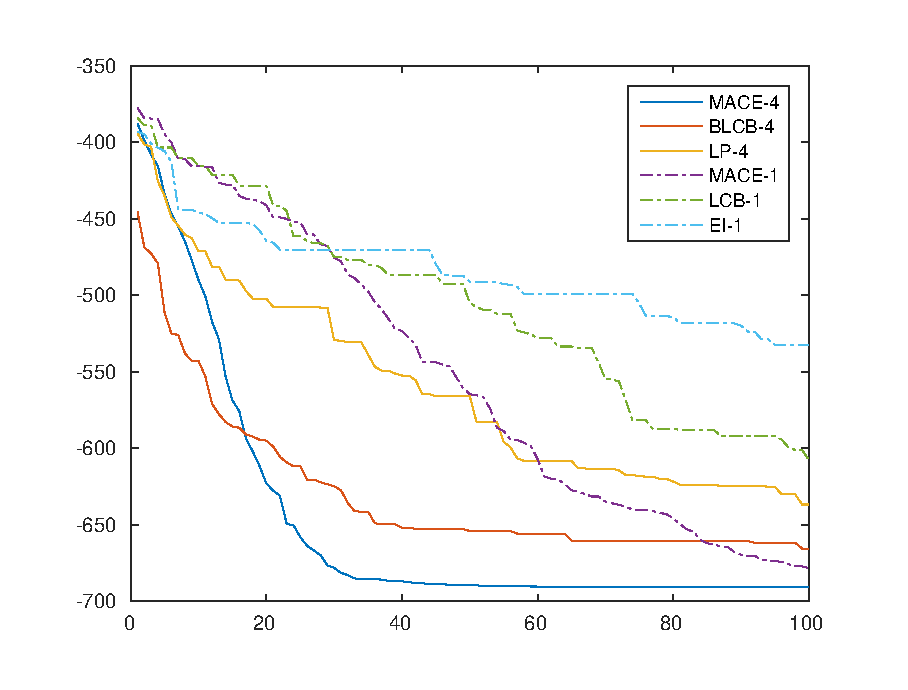
\includegraphics[width=\columnwidth]{./img/mean_DAC2014.eps}}
\caption{Optimization results of the operational amplifier}
\label{resDAC2014}
\end{center}
\vskip -0.2in
\end{figure}


\subsection{ClassE Power Amplifier}

\textcolor{red}{TODO: qKG and qEI}

\begin{figure}[htbp]
\vskip 0.2in
\begin{center}
\centerline{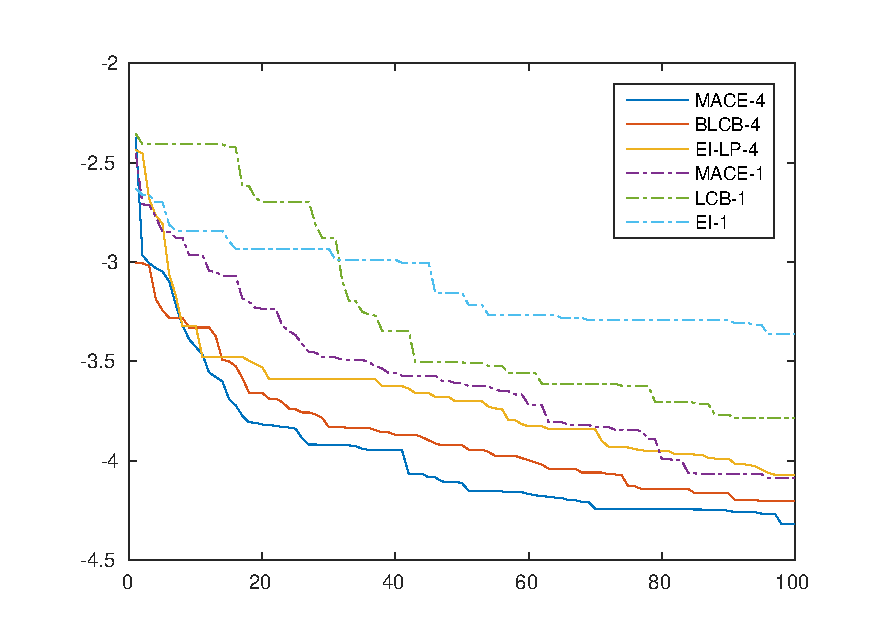
\includegraphics[width=\columnwidth]{./img/ClassE_mean.eps}}
\caption{Optimization results of the class-E power amplifier}
\label{resDAC2014}
\end{center}
\vskip -0.2in
\end{figure}


% \section{Conclusion}

In this paper, a batch Bayesian optimization algorithm is proposed for the
automation of analog circuit design. The parallelization is achieved via
the multi-objective ensemble of acquisition functions. In each iteration, the
candidate points are sampled from the Pareto front of multiple acquisition
functions. We compared the proposed MACE algorithm using analytical benchmark
functions and real-world circuits, it is shown that the MACE algorithm is
competitive compared with the state-of-the-art methods listed in the paper.


% \section*{Acknowledgements}
% This research was supported  partly by the National Major Science and
% Technology Special Project of China (2017ZX01028101-003), partly by National
% Natural Science Foundation of China (NSFC) research projects 61774045,
% 61574044, 61474026, 61574046, 61674042, and 61628402 and partly by the
% Recruitment Program of Global Experts (the Thousand Talents Plan).

%%%%%%%%%%%%%%%%%%%%%%%%%%%%%%%%%%%%%%%%%%%%%%%%%%%%%%%%%%%%%%%%%%%%%%%%%%%%%%%

\bibliography{ref}
\bibliographystyle{icml2018}


\end{document}


% This document was modified from the file originally made available by
% Pat Langley and Andrea Danyluk for ICML-2K. This version was created
% by Iain Murray in 2018. It was modified from a version from Dan Roy in
% 2017, which was based on a version from Lise Getoor and Tobias
% Scheffer, which was slightly modified from the 2010 version by
% Thorsten Joachims & Johannes Fuernkranz, slightly modified from the
% 2009 version by Kiri Wagstaff and Sam Roweis's 2008 version, which is
% slightly modified from Prasad Tadepalli's 2007 version which is a
% lightly changed version of the previous year's version by Andrew
% Moore, which was in turn edited from those of Kristian Kersting and
% Codrina Lauth. Alex Smola contributed to the algorithmic style files.
